\normaltrue \difficilefalse \tdifficilefalse
\correctiontrue
%\UPSTIidClasse{11} % 11 sup, 12 spé
%\newcommand{\UPSTIidClasse}{11}

\exer{Banc hydraulique $\star$ \label{C2:03:prec:63}}
%% CCP MP 2010
\setcounter{question}{0}\UPSTIcompetence[2]{C2-03}
\index{Compétence C2-03}
\index{Schéma-blocs}
\index{Précision}

\ifcorrection
\else
\marginnote{\textbf{Pas de corrigé pour cet exercice.}}
\fi

\ifprof
\else 

Pour limiter l’erreur statique due aux fuites, on envisage d’asservir la pression d’eau dans le tube. 
%L’objectif est ici de proposer un réglage du correcteur pour répondre aux critères du cahier des charges.
La pression d’eau à l’intérieur du tube est mesurée par un capteur de pression. 

\begin{center}
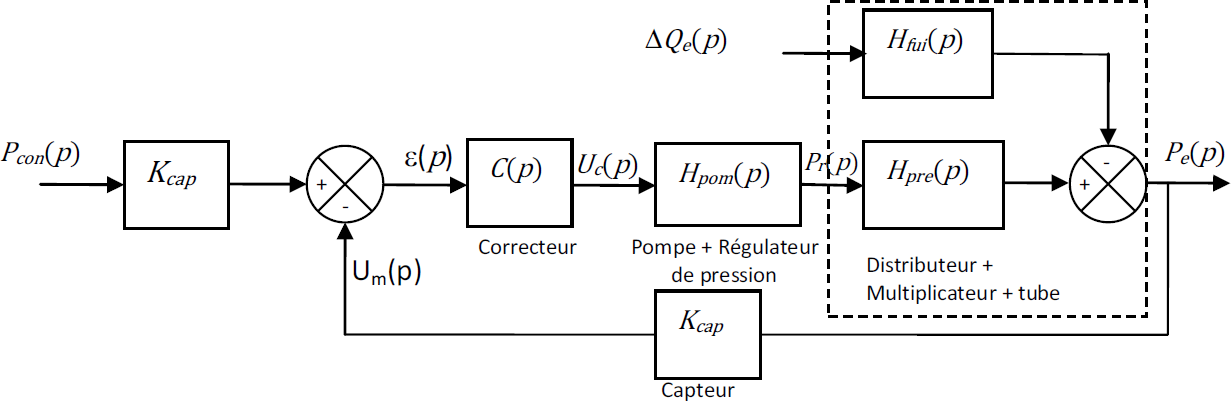
\includegraphics[width=\linewidth]{63_01}
\end{center}

 
 \begin{tabular}{lp{5cm}}
$P_{\text{con}}(p)$ : & 	pression de consigne d’eau dans le tube (Pa) \\
$P_e(p)$ : & 	pression d’eau dans le tube (Pa) \\
$U_c(p)$ : & 	tension de commande du régulateur de pression (V)\\
$P_r(p)$ : &	pression d’huile régulée (Pa)\\
$\Delta Q_e(p)$ :& 	débit de fuite (\si{m^3s^{-1}})\\
$U_m(p)$ 	:&	tension de mesure du capteur (V)\\
\end{tabular}
 
 Hypothèses :
\begin{itemize}
\item L’ensemble de mise sous pression {tube + distributeur + multiplicateur de pression} est défini par les transmittances suivantes : $H_{\text{pre}} (p)=\dfrac{K_m}{1+T_1 p}$	et	$H_{\text{fui}} (p)=\dfrac{K_f}{1+T_1 p}$ avec 	$K_m = 3,24$ ; 	$K_f = \SI{2,55e10}{Pa.m^{-3}.s}$ ; 	$T_1  = \SI{10}{s}$.
\item L’ensemble {pompe+régulateur de pression} est modélisé par la fonction de transfert :
$H_{\text{pom}} (p)=\dfrac{K_{\text{pom}}}{1+T_2 p}$  avec 	$K_{\text{pom}} = \SI{1,234e7}{Pa/V}$; 	$T_2 = \SI{5}{s}$.
\item Le capteur est modélisé par un gain pur :	$K_{\text{cap}} = \SI{2,5e-8}{V/Pa}$.
\end{itemize}
La pression de consigne est de $P_{\text{con}} = \SI{800}{bars}$ et les débits de fuite sont estimés à $\Delta Q_e = \SI{5e-4}{m3/s}$.

 
Le cahier des charges concernant le réglage de la pression de test est le suivant.
\begin{center}
\begin{tabular}{lp{5cm}}
\hline 
Stabilité :  & marge de phase de 60\degres  \\
  	  &  marge de gain de \SI{12}{dB} \\ \hline
Rapidité :  &  temps d’établissement te < 40 s \\ \hline
Précision : & 	erreur statique < 5\% soit pour une consigne de 800 bars : \\
&erreur statique due à la consigne : $\varepsilon_{\text{con}}< 5\%$  \\
& erreur statique due à la perturbation $\varepsilon_{\text{pert}} < \SI{40}{bars}$ \\ \hline
Amortissement :&	pas de dépassement \\ \hline
\end{tabular}
\end{center}

Dans le cas d’un système bouclé convenablement amorti, on pourra utiliser, sans aucune justification, la relation :
$t_e \cdot \omega_{\SI{0}{dB}}=3$ où $\omega_{\SI{0}{dB}}$ désigne la pulsation de coupure à \SI{0}{dB} en boucle ouverte et $t_e$ le temps d’établissement en boucle fermée vis-à-vis d’un échelon de consigne :
\begin{itemize}
\item $t_e = t_m$, temps du 1er maximum si le dépassement est supérieur à \SI{5}{\%},
\item $t_e = t_R$, temps de réponse à \SI{5}{\%} si le dépassement est nul ou inférieur à \SI{5}{\%}.
\end{itemize}
On envisage tout d’abord un correcteur de type proportionnel : $C(p)=K_p$. 
\fi

\question{Déterminer, en fonction de $K_p$ ,  $\varepsilon_{\text{con}}$ définie comme l’erreur statique pour une entrée consigne $P_{\text{con}}$ de type échelon, dans le cas où le débit de fuite est nul.}
\ifprof

Le débit de fuite est nul; donc $\Delta Q_e(p)=0$.

\textbf{Cas 1 : cours sur la précision connu \textit{-- Attention à avoir le même type d'entrée/sortie}}

La FTBO est de classe nulle ($C(p)$ est un gain, $H_{\text{pom}} (p)$ et $H_{\text{pre}} (p)$ de classe 0). Le gain de la Boucle ouverte est $K_{\text{BO}}=K_p K_m K_{\text{pom}}K_{\text{cap}}$.


Si l'entrée est un échelon d'amplitude $P_0$, l'écart statique est donc donné par 
$\varepsilon_S = \dfrac{P_0}{1+K_{\text{BO}}}= \dfrac{P_0}{1+K_p K_m K_{\text{pom}}K_{\text{cap}}}$.



\textbf{Cas 2 : cours sur la précision peu connu -- À savoir faire, mais on perd un peu de temps... \textit{-- Attention à avoir le même type d'entrée/sortie}}
Si on connait quand même un petit peu son cours, on a 
$\varepsilon(p)
=
\dfrac{P_{\text{con}}(p)}%
{1+K_P \dfrac{K_{\text{pom}}}{1+T_2 p} \dfrac{K_m}{1+T_1 p} K_{\text{cap}}}$.

On a alors,
$\varepsilon_s = \lim\limits_{p\to 0} p 
\dfrac{\dfrac{P_0}{p}}%
{1+K_P \dfrac{K_{\text{pom}}}{1+T_2 p} \dfrac{K_m}{1+T_1 p} K_{\text{cap}}}$
$=
\dfrac{P_0}%
{1+K_P K_{\text{pom}}K_m K_{\text{cap}}}
$

\textbf{Cas 3 : cours sur la précision pas connu -- À savoir faire, mais on perd beaucoup peu de temps...}

En utilisant la formule de Black, on a $P_e(p) 
= P_{\text{con}}(p) K_{\text{cap}} 
\dfrac{K_P \dfrac{K_{\text{pom}}}{1+T_2 p} \dfrac{K_m}{1+T_1 p} }%
{1+K_P \dfrac{K_{\text{pom}}}{1+T_2 p} \dfrac{K_m}{1+T_1 p} K_{\text{cap}}}$

$= P_{\text{con}}(p) K_{\text{cap}}(p) 
\dfrac{K_P K_{\text{pom}}K_m }%
{\left(1+T_2 p\right)\left(1+T_1 p\right)+K_P K_{\text{pom}} K_m K_{\text{cap}}}$

En passant à la valeur finale avec une entrée échelon, on a 
$\lim\limits_{t\to +\infty}P_e(t) =  P_{0} K_{\text{cap}} 
\dfrac{K_P K_{\text{pom}}K_m }%
{1+K_P K_{\text{pom}} K_m K_{\text{cap}}}$

L'écart statique est donc donné par
$
\varepsilon_S = P_0 - P_{0} 
\dfrac{K_P K_{\text{pom}}K_m K_{\text{cap}} }%
{1+K_P K_{\text{pom}} K_m K_{\text{cap}}}
= P_0
\dfrac{1+K_P K_{\text{pom}} K_m K_{\text{cap}} - K_P K_{\text{pom}}K_m K_{\text{cap}} }{1+K_P K_{\text{pom}} K_m K_{\text{cap}}}
$

$= 
\dfrac{P_0}{1+K_P K_{\text{pom}} K_m K_{\text{cap}}}$

\else 
\fi

\question{Proposer un réglage de $K_p$ pour limiter $\varepsilon_{\text{con}}$ à la valeur spécifiée dans le cahier des charges.}
\ifprof
On souhaite que l'écart statique soit inférieure à 5\% soit 0,05 pour une entrée unitaire. 

On cherche donc $K_P$ tel que 
$\dfrac{1}{1+K_P K_{\text{pom}} K_m K_{\text{cap}}}<0,05 $
$ \Leftrightarrow 1<0,05\left(1+K_P K_{\text{pom}} K_m K_{\text{cap}}\right)$

$ \Leftrightarrow \dfrac{1 - 0,05}{0,05 K_{\text{pom}} K_m K_{\text{cap}}}<K_P $

Soit $ K_P > \dfrac{1 - 0,05}{0,05 \times 1,234 \times 10^7\times 3,24 \times  2,5 \times 10^{-8}}  \Rightarrow K_P > 19$.
\else 
\fi

\question{Dans le cas où la consigne de pression est nulle,  déterminer en fonction de $K_p$ la fonction de transfert en régulation définie par : $H_{\text{pert}}(p)=\dfrac{P_e (p)}{\Delta Q_e (p)}$. En déduire, en fonction de $K_p$,  $\varepsilon_{\text{pert}}$  définie comme l’erreur statique pour une perturbation $\Delta Q_e$ de type échelon, dans le cas où la consigne de pression est nulle.}
\ifprof
Dans ce cas il n'y a pas d'intégrateur avant la perturbation échelon. Il faut savoir faire le calcul.

On peut utiliser la << lecture directe >> :
$P_e(p)= P_r(p)\indice{H}{pre} - \Delta Q_e(p) \indice{H}{fui}(p)$
$= \indice{H}{pre}(p)\indice{H}{pom}(p) C(p) \varepsilon(p)- \Delta Q_e(p) \indice{H}{fui}(p)$
$= -\indice{H}{pre}(p)\indice{H}{pom}(p) C(p) \indice{K}{cap} P_e(p)- \Delta Q_e(p) \indice{H}{fui}(p)$.

$\Leftrightarrow P_e(p) \left(1+\indice{H}{pre}(p)\indice{H}{pom}(p) C(p) \indice{K}{cap} \right)
=- \Delta Q_e(p) \indice{H}{fui}(p)$


$\Leftrightarrow \dfrac{P_e(p)}{\Delta Q_e(p)} 
=-  \dfrac{\indice{H}{fui}(p)}{1+\indice{H}{pre}(p)\indice{H}{pom}(p) C(p) \indice{K}{cap}}$


Calculons $\indice{\varepsilon}{pert}(p) = -  \dfrac{\indice{H}{fui}(p)}{1+\indice{H}{pre}(p)\indice{H}{pom}(p) C(p) \indice{K}{cap}} \Delta Q_e(p) \indice{K}{cap}$.

On a alors $\indice{\varepsilon}{pert}= \tvf{\varepsilon} 
= \lim\limits_{p\to 0} - p\times  \dfrac{\indice{H}{fui}(p)}{1+\indice{H}{pre}(p)\indice{H}{pom}(p) C(p) \indice{K}{cap}} \dfrac{\Delta Q_0}{p} \indice{K}{cap}$

$= - \dfrac{K_f\Delta Q_0 \indice{K}{cap}}{1+K_m\indice{K}{pom} K_P \indice{K}{cap}} $

\else 
\fi

\question{Proposer un réglage de $K_p$ pour limiter $\varepsilon_{\text{pert}}$ à la valeur spécifiée au cahier des charges.}
\ifprof
Pour $\Delta Q_e = \SI{5e-4}{m^3.s^{-1}}$, il faut $\indice{\varepsilon}{pert}<40\times 10^5$ (Pa) soit

$\dfrac{K_f\Delta Q_0 \indice{K}{cap} }{1+K_m\indice{K}{pom} K_P \indice{K}{cap}}  < 40\times 10^5$
$\Rightarrow  K_f\Delta Q_0 \indice{K}{cap}  < 40\times 10^5\left(1+K_m\indice{K}{pom} K_P \indice{K}{cap}\right)$
$\Rightarrow \dfrac{K_f\Delta Q_0 \indice{K}{cap}  -40\times 10^5}{40\times 10^5 K_m\indice{K}{pom} \indice{K}{cap} }< K_P $
$\Rightarrow K_P > -1$
\else 
\fi

\question{Proposer un réglage de $K_p$ pour vérifier le critère d’amortissement. Conclure quant au choix d’un correcteur proportionnel.}
\ifprof
Je vous laisse faire le calcul... Il faut savoir le faire le plus vite possible.
Il faut d'abord calculer la FTBF, la mettre sous forme canonique, déterminer 
$\indice{\xi}{BF}=\dfrac{T_1+T_2}{2\sqrt{T_1T\left( 1+K_P K_M \indice{K}{Pom}\indice{K}{Cap}\right)}}$ puis
determiner $K_P$ tel que $\indice{\xi}{BF}=1$.

\else 
\fi
 

\ifprof
\else

\noindent\footnotesize
\fbox{\parbox{.9\linewidth}{
Éléments de corrigé : 
\begin{enumerate}
  \item $\varepsilon_{\text{con \%}} = \dfrac{1}{1+K_PK_m K_{\text{pom}} K_{\text{cap}} }$;
  \item $K_P > 19$;
  \item $\varepsilon_{\text{pert}} = \Delta Q_e \dfrac{K_f}{1+K_{\text{cap}}K_PK_mK_{\text{pom}}}$;
  \item $K_P > -1$.% $K_P > 2,19$.
  \item $K_P < 0,125$. Il est impossible de vérifier les trois conditions avec un correcteur proportionnel.
\end{enumerate}}}
\normalsize

\begin{flushright}
\footnotesize{Corrigé  voir \ref{C2:03:prec:63}.}
\end{flushright}%
\fi